\documentclass{article}%
\usepackage{amsmath}%
\usepackage{amsfonts}%
\usepackage{amssymb}%
\usepackage{enumerate}% http://ctan.org/pkg/enumerate
\usepackage{tikz}
\usepackage{graphicx}
\usepackage{qtree}
\usepackage{enumit  em}
\usepackage{bm}
\usepackage{changepage} 
\usepackage{multicol}
\usepackage{subfig}
\usepackage{float}
\usepackage{placeins}
\usepackage[toc,page]{appendix}
% code 
\usepackage{listings, color}
\usepackage{minted}
%-------------------------------------------
\newtheorem{theorem}{Theorem}
\newtheorem{algorithm}[theorem]{Algorithm}
\newtheorem{claim}[theorem]{Claim}
\newtheorem{proposition}[theorem]{Proposition}
\newtheorem{corollary}[theorem]{Corollary}
\newtheorem{definition}[theorem]{Definition}
\newtheorem{notation}[theorem]{Notation}
\newtheorem{example}[theorem]{Example}
\newtheorem{exercise}[theorem]{Exercise}
\newtheorem{lemma}[theorem]{Lemma}
\newtheorem{remark}[theorem]{Remark}
\newtheorem{solution}[theorem]{Solution}
\newenvironment{proof}[1][Proof]{\textbf{#1.} }{\ \rule{0.5em}{0.5em}}

% code
\definecolor{dkgreen}{rgb}{0,0.6,0}
\definecolor{gray}{rgb}{0.5,0.5,0.5}
\definecolor{mauve}{rgb}{0.58,0,0.82}

\lstset{frame=tb,
  language=Java,
  frame = trBL,
  aboveskip=3mm,
  belowskip=3mm,
  showstringspaces=false,
  columns=flexible,
  basicstyle={\small\ttfamily},
  numbers=none,
  numberstyle=\tiny\color{gray},
  keywordstyle=\color{blue},
  commentstyle=\color{dkgreen},
  stringstyle=\color{mauve},
  breaklines=true,
  breakatwhitespace=true,
  tabsize=3
}

\setlength{\textwidth}{7.0in}
\setlength{\oddsidemargin}{-0.35in}
\setlength{\topmargin}{-0.5in}
\setlength{\textheight}{9.0in}
\setlength{\parindent}{0pt}
% \setlength{\parskip}{0.25cm}
\linespread{1.4}

% DEFINING COMMAND SHORTCUTS
\def\<{\langle}
\def\>{\rangle}

% NEW COMMANDS
\newcommand{\bigO}[1]{$O(#1)$}

\begin{document}

% ======================================================================== %

\pagenumbering{gobble} % Disable page number on title page
\begin{titlepage}
    \centering
	\vspace*{\stretch{0.5}}
    % \vfill
	{\scshape\Large ECSE 420 - Parallel Computing \par}
	\vspace{5mm}
	{\huge\bfseries Assignment 3 \par}
	

	\vfill
	
	{\large Arian Omidi - 260835976\par}
	{\large{Namdar Nejad - 260893536}\par}
	\vspace{10mm}
	{\large \today\par}
	
	\vfill
\end{titlepage}

\pagenumbering{arabic} % Set page numbering to Arabic numbers
\setcounter{page}{1} % Set page number to 1

% ======================================================================== %

\section{Memory Access \& Anderson Lock}
    \subsection{}
        Since the average time per access remains constant in the green graph, we can conclude that we are fetching each element of the array from the memory and are able to store it in the cache without doing extra operations (write, replace, … due to the cache misses). So $L’$ represents the size of the cache which is 4 words here and $t_0$ is the average access time to the array that is entirely in the memory.
    
    \subsection{}
        If the array size is bigger than the cache size, we will be facing cache misses at some points. So $t_1$ is the average access time to the array when fetching elements that are not in the cache.

    \subsection{} 
        \begin{enumerate}[label=\textbf{Part \arabic*:},leftmargin=*,align=left]
        % \baselineskip=1pt
            \item The entire array can fit into the cache and we have an empty cache so the access time is constant and rather small.
            
            \item In this case, we are slowly facing cache misses and the access time is not constant. As the stride increase so does the access time.
            
            \item In this section, we have reached a point where the cache is entirely full and we are only having cache misses. So the access time is constant but quite high.
        \end{enumerate}
     
    \subsection{}  
        Using the padding technique would increase the cache misses as we would be filling the cache with extra data that is not useful, thus degrading the overall performance of the lock.
        
\section{Examining the Fine-Grained Algorithm}
    \subsection{Contains Implementation}
        The implementation for the \mintinline{bash}{contains()} can be found in \mintinline{bash}{Q2Contains.java} below in \textbf{Appendix \ref{q2-contains}}. \\
        
        The fine-grained algorithm described in Chapter 9.5 improves concurrency by locking individual nodes instead of the entire list. We need a “lock coupling” protocol to do our operations on the list. In the \mintinline{bash}{contains()} method, we iterate through the list until we find the key we are looking for, and check at each step compare it with the key of the node.
        
    \subsection{Test Implementation}
        The test code can be found in \mintinline{bash}{Q2Test.java} below in \textbf{Appendix \ref{q2-test}}. \\
        
        In the test method we create a number of threads that add a certain number of items to the list. After completing the list we check if it contain a given element and print the result.

        
\section{Bounded Queue} 
    \subsection{Lock-Based Queue}
    The lock-based bounded queue implementation can be found below in \textbf{Appendix \ref{queue}} under \mintinline{bash}{BoundedQueue.java}.
    
    \subsection{Lock-Free Queue}
    The lock-free bounded queue implementation can be found below in \textbf{Appendix \ref{lock-free-queue}} under \mintinline{bash}{LockFreeBoundedQueue.java}.\\
    
    We ran into difficulties defining the criteria for allowing queuing and dequeuing as we had to ensure that the data was not being overwritten. To overcome this challenge, we made all of the pointers and the array into Atomic Objects as well as adding another Atomic Integer to keep track of the current size. 
    


\section{Matrix Vector Multiplication}
    \subsection{Sequential Implementation}
        The sequential multiplication implementation can be found below in \textbf{Appendix \ref{seq-mult}} under \mintinline{bash}{SequentialMultiplier.java}.\\
        
        The naive sequential matrix-vector multiplication was implemented by calculating the dot product between each row of the matrix and the vector. Thus, this method achieves a \bigO{n^2} runtime complexity. 
    
    \subsection{Parallel Implementation}
        The highly parallel and practical parallel multiplication implementations can be found below in \textbf{Appendix \ref{q4}} under \mintinline{bash}{ParallelMultiplier.java} and \mintinline{bash}{PracticalParallelMultiplier.java} respectively.\\
        
        For the parallel matrix-vector multiplication we implemented two different methods: a highly parallel multiplier and a practical parallel multiplier. As the name suggests the highly parallel multiplier, has a $\Theta(\log{n})$ critical path. However, a side-effect of its high parallelism is that it need many processors to achieve this performance. Since at each step the algorithm must create 2 new threads, the overhead of this method is huge. Thus, while this approach is theoretically optimal, in practice it is orders of magnitude slower than the sequential multiplier.\\
        
        To remedy this, we implemented a practical parallel multiplier which uses the simple methods we implemented in Assignment 1 to greatly speed up the performance of matrix-vector multiplication. 
        
    
    \subsection{Sequential vs Parallel Comparison}
        Since our highly parallel multiplier crashes our computers when multiplying matrices of size 200, we used our practical parallel multiplier for this comparison.\\
        
        \begin{figure}[H]
            \centering
            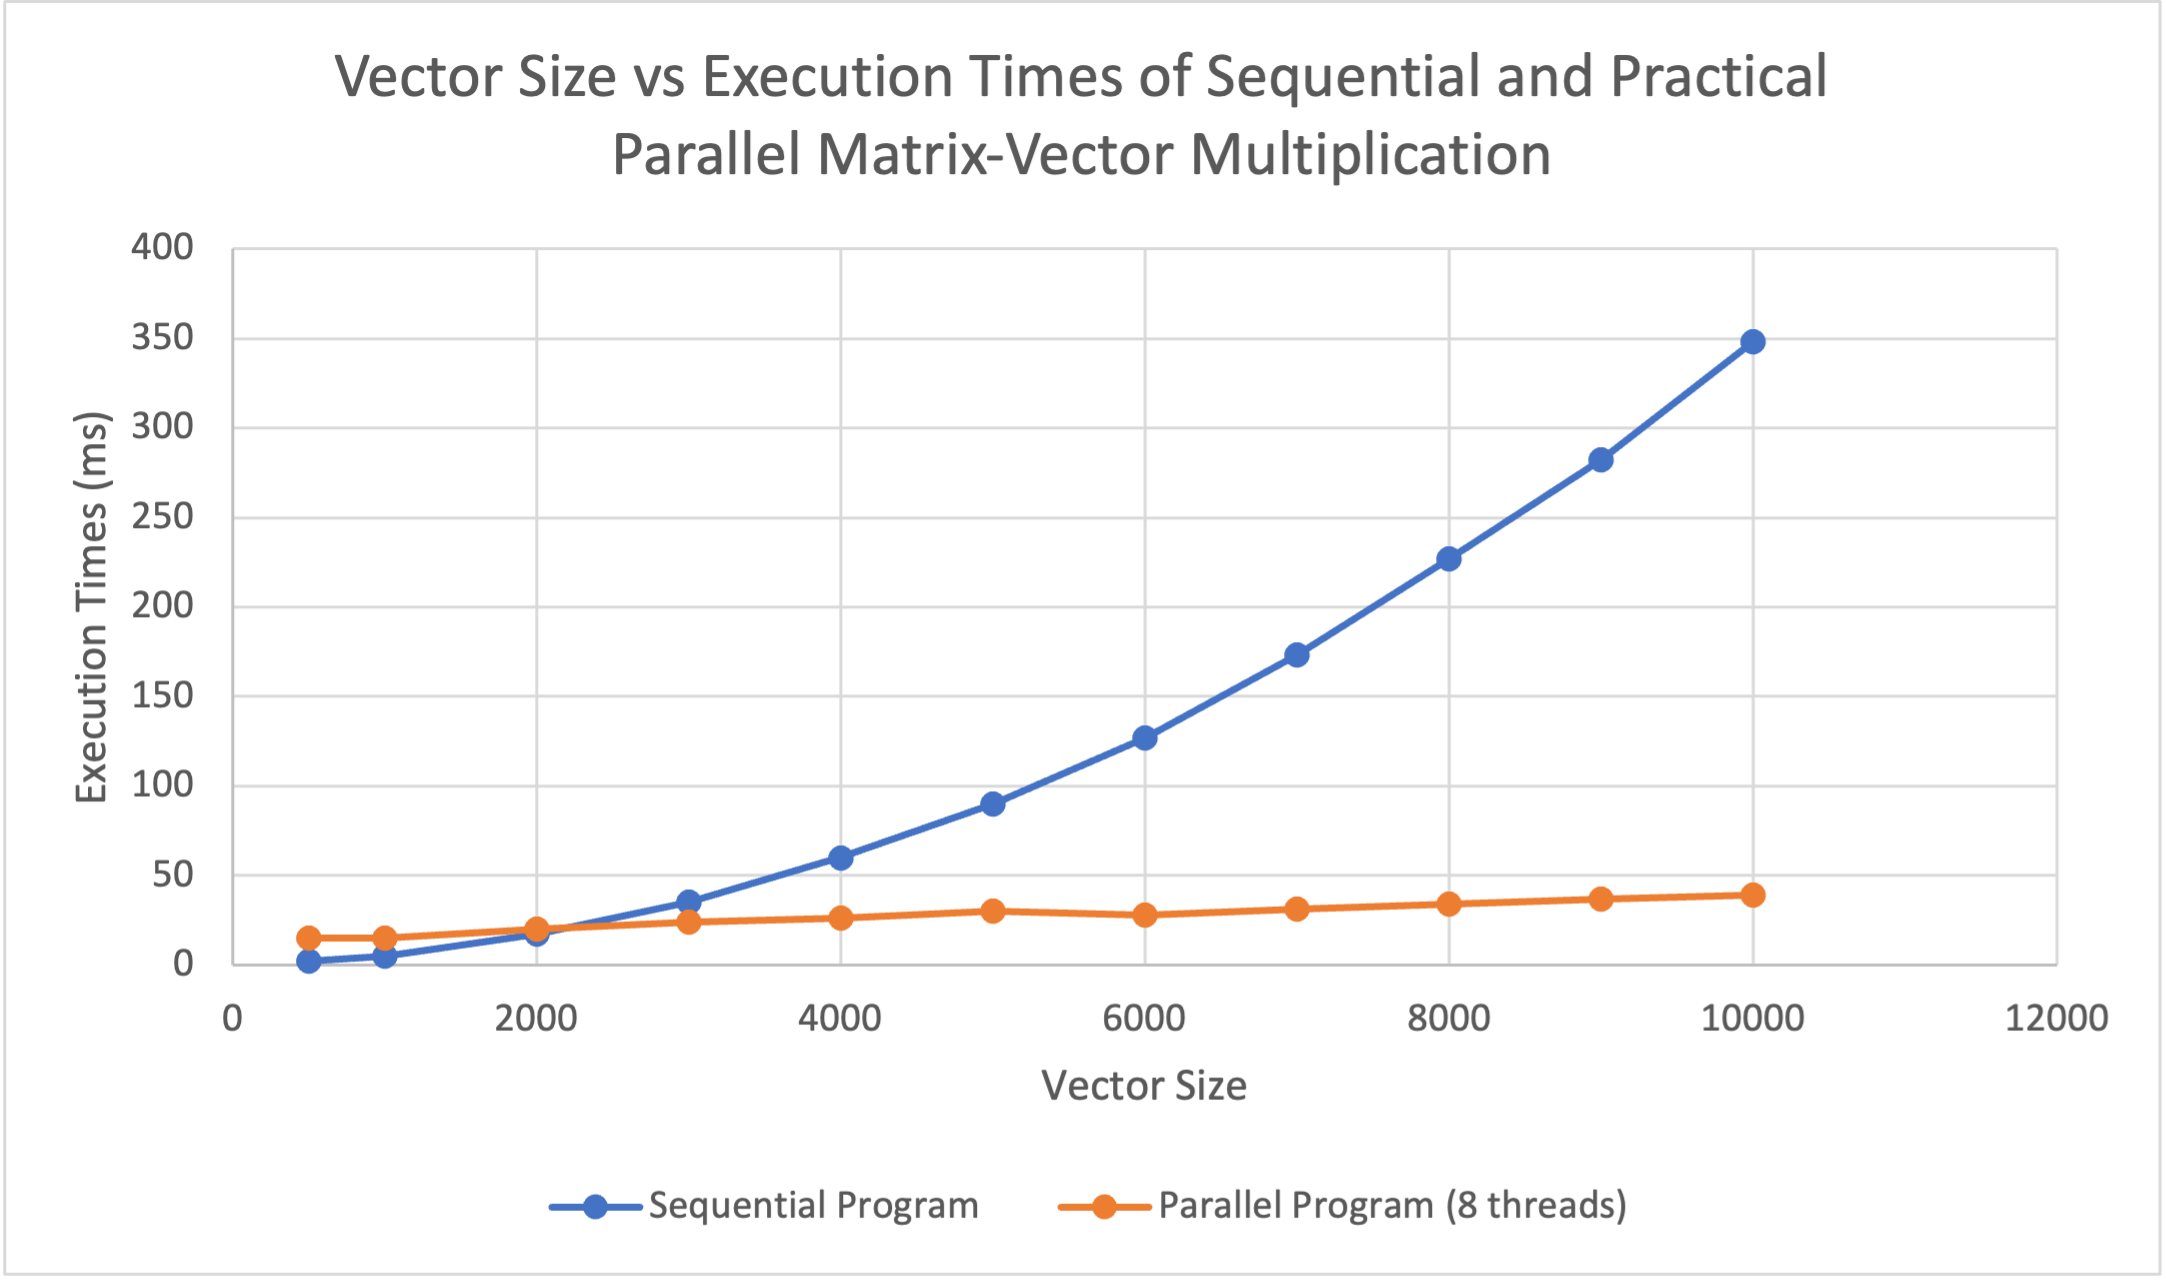
\includegraphics[width=0.6\textwidth]{images/times.png}
            \caption{Vector size vs. Execution time}
        \end{figure}
        \FloatBarrier
        
        As seen in Figure 1, we compared the execution time of the sequential and parallel multipliers, running on 8 threads, with differing vector sizes. We observed that with a vector size, $N$, less than 2000, the sequential multiplier was more efficient due to its minimal overhead. However, for $N > 2000$, the parallel multiplier greatly outperformed the sequential multiplier which grew at and exponential level. \\
        
        At around $N = 2000$, the two methods converged and produced similar execution times, with the sequential multiplier finishing in 17ms while the parallel multiplier finished in 20ms. Thus, as observed in Figure 2, the speed up at $N = 2000$ is equal to 0.85. 
        
        \begin{figure}[H]
            \centering
            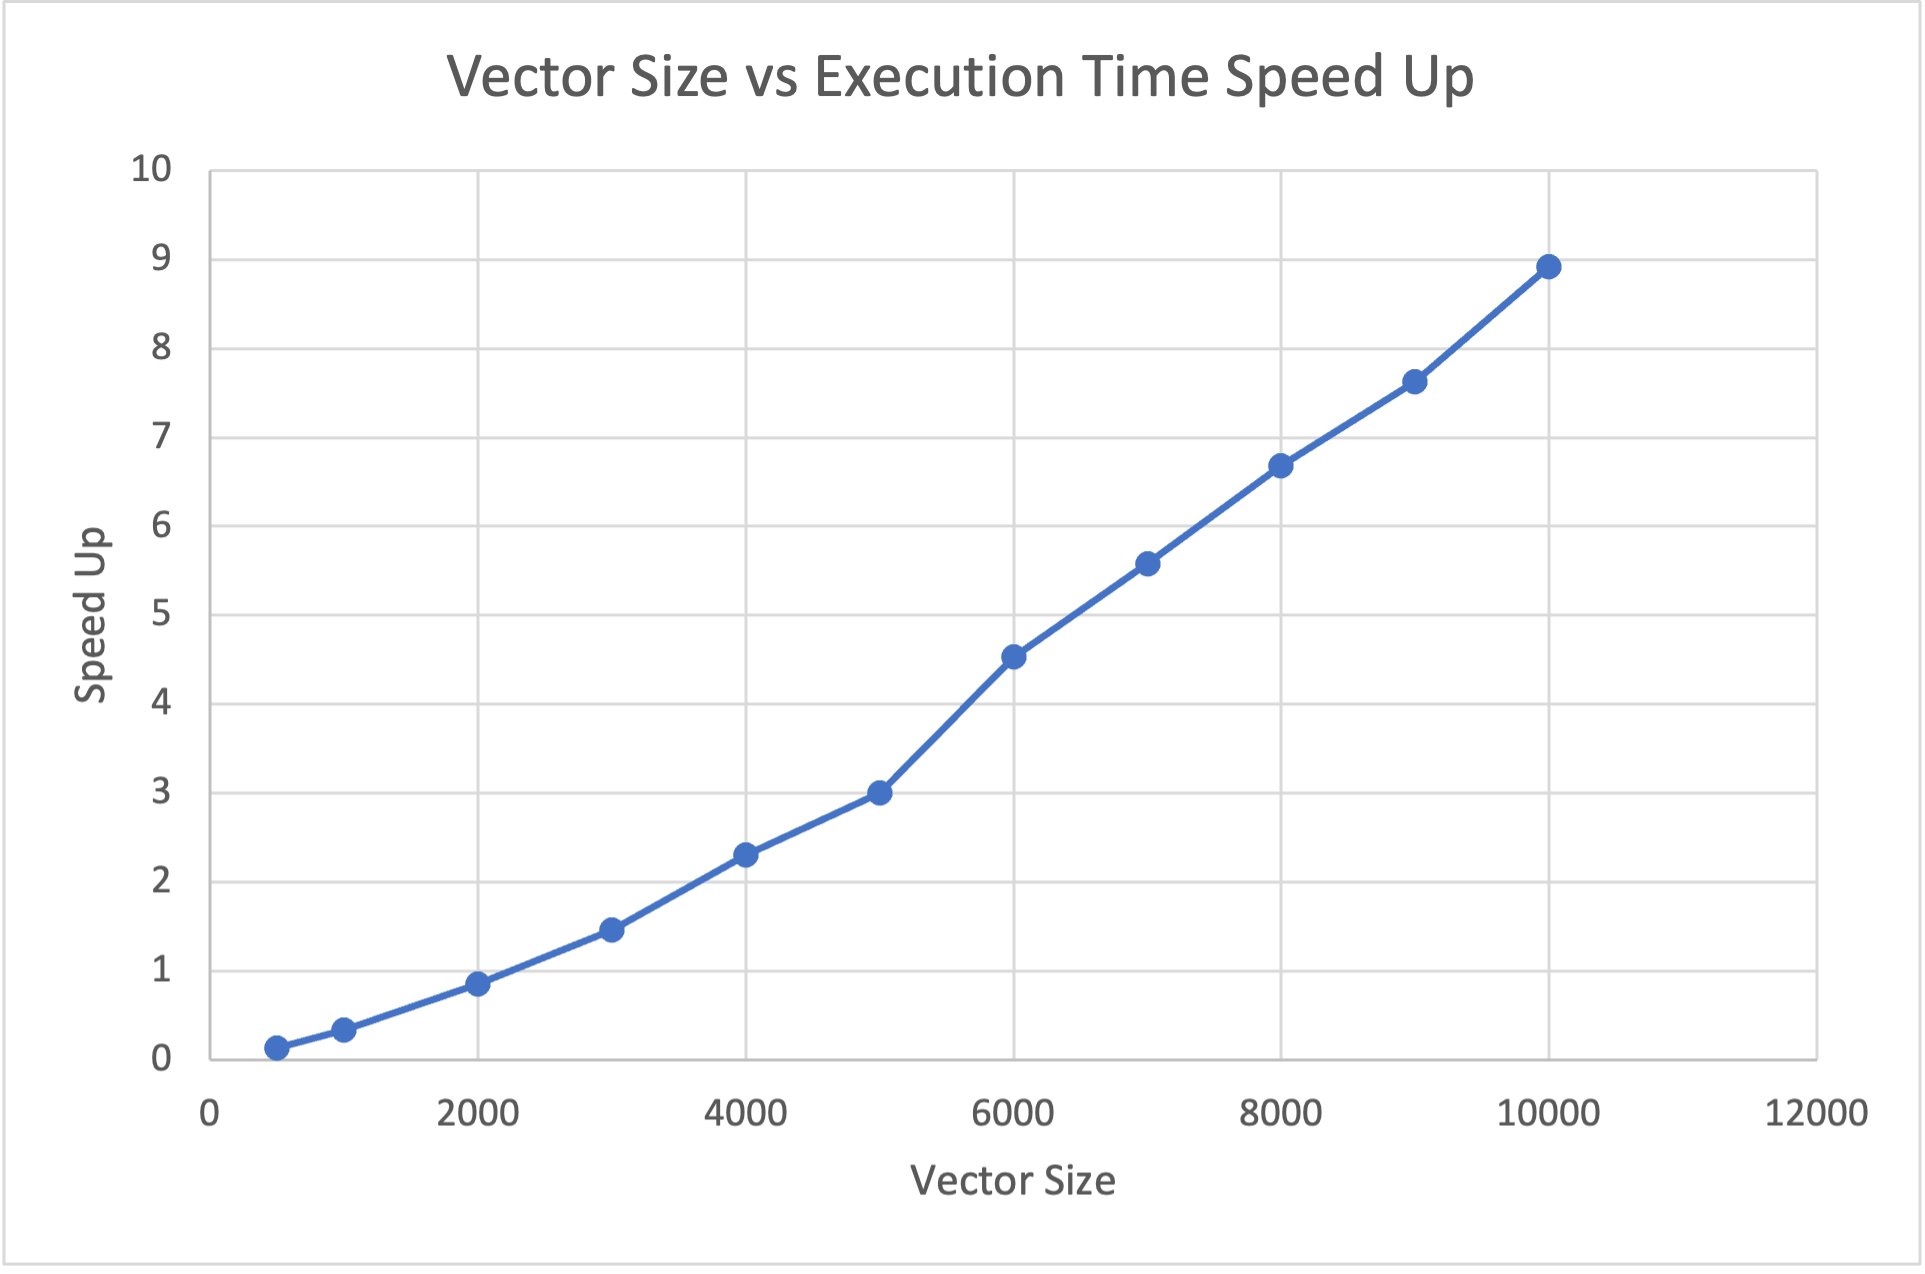
\includegraphics[width=0.6\textwidth]{images/speed-up.png}
            \caption{Vector size vs. Execution time speed up}
        \end{figure}
        \FloatBarrier

    \subsection{Work and Critical Path}
        The highly parallel multiplier leverages the fact that if $C = M \cdot V$ then 
        \begin{gather}
            \begin{pmatrix} C_0 \\ C_1 \end{pmatrix}
            =
            \begin{pmatrix} M_{00} & M_{01} \\ M_{10} & M_{11} \end{pmatrix}
            \begin{pmatrix} V_0 \\ V_1 \end{pmatrix}
            = 
            \begin{pmatrix} M_{00} \cdot V_0 + M_{01} \cdot V_1 \\ M_{10} \cdot V_0 + M_{11} \cdot V_1  \end{pmatrix}
        \end{gather}
        
        Therefore, at each step we are halving the vector and halving the matrix in two dimensions. Thus we will have $\Theta(N) \cdot \Theta(N) +  \Theta(N) = \Theta(N^2)$ work nodes from dividing the problem to the base case of one element times one element. The critical path is only $\Theta(\log_2{N})$ as we are halving the size of the vector at each step. Thus, it will only take $\log_2{N}$ steps to reach the base case.\\
        
        Since the work is $\Theta(N^2)$ and the critical path is $\Theta(\log_2{N})$, the parallelism is equal to $\Theta(\frac{N^2}{\log_2{N}})$. Since $N^2$ grows much faster than $\log_2{N}$, as $N$ gets larger the program can become nearly completley parallel. 
        
    
    
\newpage  
\begin{appendices}
    % \renewcommand{\thesection}{\arabic{section}}
    \section{Question 2 Code}\label{q2}
    
        \subsection*{Q2Contains.java}\label{q2-contains}
        \lstinputlisting[caption=]{src/Q2Contains.java}
        
        \subsection*{Q2Test.java}\label{q2-test}
        \lstinputlisting[caption=]{src/Q2Test.java}
    
    \section{Question 3 Code}\label{q3}
    
        \subsection*{BoundedQueue.java}\label{queue}
        \lstinputlisting[caption=]{src/BoundedQueue.java}
        
        \subsection*{LockFreeBoundedQueue.java}\label{lock-free-queue}
        \lstinputlisting[caption=]{src/LockFreeBoundedQueue.java}
        
    \section{Question 4 Code}\label{q4}
    
        \subsection*{Matrix.java}\label{matrix}
        \lstinputlisting[caption=]{src/Matrix.java}
        
        \subsection*{Vector.java}\label{vector}
        \lstinputlisting[caption=]{src/Vector.java}
        
        \subsection*{SequentialMultiplier.java}\label{seq-mult}
        \lstinputlisting[caption=]{src/SequentialMultiplier.java}
        
        \subsection*{PracticalParallelMultiplier.java}\label{par-mult}
        \lstinputlisting[caption=]{src/ParallelMultiplier.java}
        
        \subsection*{PracticalParallelMultiplier.java}\label{prac-par-mult}
        \lstinputlisting[caption=]{src/PracticalParallelMultiplier.java}
        
        \subsection*{MatrixVectorMultiplication.java}\label{mult}
        \lstinputlisting[caption=]{src/MatrixVectorMultiplication.java}


\end{appendices}


\end{document}